\chapter{エディタ}
\label{chap:editor}

% この章で学ぶこと
\begin{goalbox}
  \begin{itemize}
    \item テキストエディタとは何か、なぜプログラミングに必要なのか
    \item ターミナルで使えるエディタ（nano・Vim・Emacs）の最低限の操作
    \item VS Code のインストールと、拡張機能を使った開発環境の整え方
    \item VS Code を使って、ロボットの PC やコンテナの中のファイルを編集する方法
  \end{itemize}
\end{goalbox}

プログラムや設定ファイルを書くには、\textbf{テキストエディタ}（以下、エディタ）が必要です。
エディタは、エンジニアが一日の中で最も長い時間使う道具といってもよいでしょう。
この章では、ロボット開発でよく使われる 4 つのエディタ、nano・Vim・Emacs・VS Code を紹介します。

\section{エディタとは}
\label{sec:editor-intro}

\subsection{テキストファイルとエディタ}

Word のような文書作成ソフト（ワープロ）で作ったファイルには、文字のほかに、文字の大きさや色、レイアウトといった情報も含まれています。
一方、プログラムや設定ファイルは、文字だけでできた\textbf{テキストファイル}です。
テキストファイルを作ったり編集したりするためのソフトウェアが、エディタです。

プログラムを書くためのエディタには、次のような便利な機能があります。

\begin{itemize}
  \item プログラムの文法に合わせて色を付けて表示する（シンタックスハイライト）
  \item インデント（行頭の字下げ）を自動で整える
  \item 関数名や変数名を途中まで入力すると、残りを補ってくれる（補完）
  \item 複数のファイルをまとめて検索・置換する
\end{itemize}

\subsection{ターミナルエディタと GUI エディタ}

エディタは、大きく 2 つに分けられます。

\begin{description}
  \item[ターミナルエディタ]
    ターミナルの中で動くエディタです（nano、Vim、Emacs など）。
    GUI のない環境でも使えるので、SSH でロボットにログインしたとき（\ref{chap:network}章）や、Docker のコンテナの中（\ref{chap:docker}章）で設定ファイルを少し書き換えたいときに欠かせません。
  \item[GUI エディタ]
    ウィンドウを開いて、マウスも使って操作するエディタです（VS Code など）。
    画面が見やすく、多くの機能を直感的に使えるので、ふだんのプログラミングではこちらが中心になります。
\end{description}

本書では、ふだんの開発には VS Code を使い、ターミナルで少しだけ編集したいときには nano か Vim を使う、という使い分けをおすすめします。

\section{nano}
\label{sec:editor-nano}

\textbf{nano} は、操作が簡単で、初めての人でも迷わずに使えるターミナルエディタです。
Ubuntu には最初からインストールされています。
\cmd{nano} の後ろに編集したいファイル名を指定して起動します（ファイルがなければ、新しく作られます）。

\begin{terminal}[nano でファイルを開く]
$ nano memo.txt
\end{terminal}

nano を起動すると、画面の上部にファイル名、下部に操作方法の一覧が表示されます。
下部の \cmd{\textasciicircum O} のような表示は、\cmd{\textasciicircum} が \key{Ctrl} キーを表していて、\cmd{\textasciicircum O} は \key{Ctrl}+\key{O} という意味です。
あとは、ふつうのエディタと同じように、矢印キーでカーソルを動かして文字を入力するだけです。

\begin{center}
  \begin{tabular}{ll}
    \toprule
    キー & 動作 \\
    \midrule
    \key{Ctrl}+\key{O} → \key{Enter} & 保存する \\
    \key{Ctrl}+\key{X} & 終了する（未保存なら保存するか聞かれる） \\
    \key{Ctrl}+\key{W} & 文字列を検索する \\
    \key{Ctrl}+\key{K} & 今の行を切り取る \\
    \key{Ctrl}+\key{U} & 切り取った行を貼り付ける \\
    \bottomrule
  \end{tabular}
\end{center}

\cmd{git commit} を \cmd{-m} なしで実行したときなど、コマンドがエディタを開いてくることがあります（\ref{sec:git-basic}節）。
Ubuntu では、この「標準のエディタ」も初期設定では nano になっています。

\section{Vim}
\label{sec:editor-vim}

\subsection{Vim とは}

\textbf{Vim}（ヴィム）は、1970 年代に UNIX 用に作られた vi というエディタを改良したものです。
キーボードから手を離さずに高速に編集できるように工夫されていて、今も多くのエンジニアに愛用されています。
また、vi（またはその仲間）は、ほとんどすべての Linux のコンピュータに入っているので、最低限の操作を覚えておくと、どこへ行っても困りません。
Ubuntu には最小限の機能の Vim が入っていて、\cmd{vi} コマンドで起動できます。
すべての機能を使うには、次のようにインストールします。

\begin{terminal}[Vim をインストールする]
$ sudo apt install vim
$ vim memo.txt
\end{terminal}

\subsection{モード}

Vim の最大の特徴は、\textbf{モード}があることです（図\ref{fig:editor-vim-modes}）。
Vim を起動すると、最初は\textbf{ノーマルモード}になっています。
ノーマルモードでは、キーを押しても文字は入力されず、キーの 1 つ 1 つが「カーソルの移動」「行の削除」といった命令になります。
文字を入力するには、\key{i} を押して\textbf{インサートモード}に切り替えます。
入力が終わったら、\key{Esc} でノーマルモードに戻ります。
保存や終了は、ノーマルモードで \key{:} を押して\textbf{コマンドラインモード}に入り、命令を入力して \key{Enter} を押します。

\begin{figure}[tb]
  \centering
  % 図：Vim のモードの切り替え（chapters/tools/editor.tex）
\begin{tikzpicture}[
    >=Stealth, auto, node distance=28mm and 46mm, on grid,
    every state/.style={draw, rounded corners, rectangle, fill=blue!6,
      minimum width=26mm, minimum height=11mm, font=\small, align=center}]
  \node[state, initial, initial where=above, initial text={\footnotesize 起動}, fill=blue!15] (normal) {\textbf{ノーマルモード}\\{\footnotesize 移動・コピー・削除}};
  \node[state, right=of normal, fill=green!8] (insert) {\textbf{インサートモード}\\{\footnotesize 文字を入力する}};
  \node[state, below=of normal, fill=orange!10] (cmd) {\textbf{コマンドライン}\\\textbf{モード}\\{\footnotesize 保存・終了など}};
  \path[->, thick]
    (normal) edge[bend left=20]  node[font=\footnotesize]{\texttt{i}} (insert)
    (insert) edge[bend left=20]  node[font=\footnotesize]{\texttt{Esc}} (normal)
    (normal) edge[bend left=30]  node[font=\footnotesize]{\texttt{:}} (cmd)
    (cmd)    edge[bend left=30]  node[font=\footnotesize, align=right]{\texttt{Enter}（実行）\\\texttt{Esc}（取り消し）} (normal);
\end{tikzpicture}

  \caption{Vim のモードの切り替え}
  \label{fig:editor-vim-modes}
\end{figure}

\subsection{これだけは覚えたい操作}

初めて Vim を開いた人の多くがつまずくのが、「文字が入力できない」「終了の仕方がわからない」の 2 つです。
まずは、次の操作だけ覚えておきましょう。
迷ったら、まず \key{Esc} を押してノーマルモードに戻るのが基本です。

\begin{center}
  \begin{tabular}{ll}
    \toprule
    操作（ノーマルモードで） & 動作 \\
    \midrule
    \key{i} & インサートモードに入る（カーソルの位置から入力） \\
    \key{Esc} & ノーマルモードに戻る \\
    \cmd{:w} → \key{Enter} & 保存する \\
    \cmd{:q} → \key{Enter} & 終了する \\
    \cmd{:wq} → \key{Enter} & 保存して終了する \\
    \cmd{:q!} → \key{Enter} & 保存せずに終了する \\
    \bottomrule
  \end{tabular}
\end{center}

慣れてきたら、ノーマルモードの便利な命令も使ってみましょう。
\key{h} \key{j} \key{k} \key{l} で左・下・上・右にカーソルを移動、\key{d}\key{d} で 1 行削除、\key{y}\key{y} で 1 行コピー、\key{p} で貼り付け、\key{u} で元に戻す、\cmd{/文字列} で検索、といった操作ができます。
Vim をインストールすると、\cmd{vimtutor} というコマンドで、30 分ほどで基本操作を練習できるチュートリアルを始められます。

\section{Emacs}
\label{sec:editor-emacs}

\subsection{Emacs とは}

\textbf{Emacs}（イーマックス）も、1970 年代から使われている歴史のあるエディタです。
現在広く使われている GNU Emacs は、GNU プロジェクト（\ref{sec:linux-history}節）を始めた Richard Stallman が作ったものです。
Emacs Lisp というプログラミング言語で機能を追加したり、動きを変えたりできるのが最大の特徴で、エディタの中でメールを読んだり、ファイルを管理したり、予定を管理したりと、あらゆることをこなす人もいます。

Emacs は、次のようにインストールします。
\cmd{emacs} で起動すると GUI のウィンドウが開き、\cmd{emacs -nw} で起動するとターミナルの中で動きます。

\begin{terminal}[Emacs をインストールする]
$ sudo apt install emacs
$ emacs -nw memo.txt
\end{terminal}

\subsection{基本操作}

Emacs には Vim のようなモードの切り替えはなく、起動するとすぐに文字を入力できます。
保存や終了などの操作は、\key{Ctrl} キーや \key{Alt} キーと組み合わせたキーで行います。
Emacs の説明では、\key{Ctrl}+\key{X} を \cmd{C-x}、\key{Alt}+\key{X} を \cmd{M-x} のように書くのが習慣です。
\cmd{C-x C-s} は、\key{Ctrl}+\key{X} を押した後に \key{Ctrl}+\key{S} を押す、という意味です。

\begin{center}
  \begin{tabular}{lll}
    \toprule
    Emacs での表記 & キー & 動作 \\
    \midrule
    \cmd{C-x C-f} & \key{Ctrl}+\key{X} → \key{Ctrl}+\key{F} & ファイルを開く \\
    \cmd{C-x C-s} & \key{Ctrl}+\key{X} → \key{Ctrl}+\key{S} & 保存する \\
    \cmd{C-x C-c} & \key{Ctrl}+\key{X} → \key{Ctrl}+\key{C} & 終了する \\
    \cmd{C-s} & \key{Ctrl}+\key{S} & 文字列を検索する \\
    \cmd{C-g} & \key{Ctrl}+\key{G} & 操作を取り消す（困ったらこれ） \\
    \bottomrule
  \end{tabular}
\end{center}

\cmd{C-h t}（\key{Ctrl}+\key{H} → \key{T}）で、Emacs の使い方を学べるチュートリアルが始まります。

\begin{point}[シェルのキー操作は Emacs 流]
  \ref{sec:terminal-keys}節で紹介した、\key{Ctrl}+\key{A}（行頭へ移動）、\key{Ctrl}+\key{E}（行末へ移動）、\key{Ctrl}+\key{K}（カーソルより後ろを削除）といったシェルのキー操作は、実は Emacs のキー操作と同じです。
  bash は、標準で Emacs と同じキー操作で編集できるようになっているのです。
  これらのキー操作に慣れておくと、ターミナルでも Emacs でも役に立ちます。
\end{point}

\section{VS Code}
\label{sec:editor-vscode}

\subsection{VS Code とは}

\textbf{Visual Studio Code}（VS Code）は、Microsoft が開発している無料の GUI エディタです。
軽快に動作し、Python や C++ をはじめ、ほとんどのプログラミング言語に対応しています。
\textbf{拡張機能}を追加することで、さまざまな機能を後から付け加えられるのが特徴で、近年、最も広く使われているエディタの 1 つです。
ROS 2 の開発でも、多くの人が VS Code を使っています。

\subsection{インストール}

VS Code は、公式サイト（\url{https://code.visualstudio.com/}）から Ubuntu 用の \cmd{.deb} ファイルをダウンロードし、\cmd{apt} でインストールします（\ref{sec:package-apt}節）。
インストールすると、VS Code の公式リポジトリも自動で登録されるので、以降は \cmd{sudo apt upgrade} で最新の版に更新できます。

\begin{terminal}[VS Code をインストールする]
$ cd ~/Downloads
$ sudo apt install ./code_1.93.1_amd64.deb
\end{terminal}

ファイル名の数字（バージョン）は、ダウンロードした時期によって変わります。

\subsection{起動と画面の構成}

VS Code は、アプリケーションの一覧から起動できるほか、ターミナルから \cmd{code} コマンドで起動できます。
\cmd{code .} と入力すると、カレントディレクトリをまるごと開いた状態で起動します。
プロジェクトのディレクトリに \cmd{cd} で移動してから \cmd{code .} で開く、という使い方が便利です。

\begin{terminal}[プロジェクトのディレクトリを VS Code で開く]
$ cd ~/my_robot
$ code .
\end{terminal}

VS Code の画面は、主に次の部分でできています（図\ref{fig:editor-vscode}）。

\begin{figure}[tb]
  \centering
  \large
  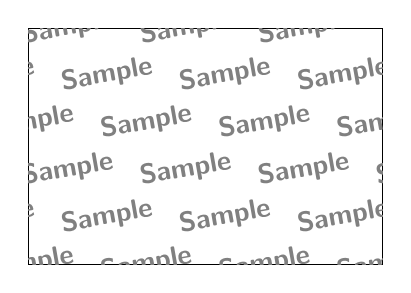
\begin{tikzpicture}
    \draw rectangle++(4.5,3);
    \clip rectangle++(4.5,3);
    \foreach\x in{0,1,2,3,4}{
      \foreach\y in{0,1,2,3,4,5,6}{
        \path(\x*1.5-\y*0.5,\y*0.6)node[rotate=10,text=gray]{\sffamily\bfseries\itshape Sample };
      }
    }
  \end{tikzpicture}
  %% 入れる画像：VS Code で ~/my_robot を開き、エクスプローラーにファイル一覧、エディタに README.md、下部に統合ターミナルを表示した状態のスクリーンショット（各部分に番号を付ける）
  % eps 画像を貼る場合は includegraphics をお使いください。
  % \includegraphics[width=0.8\linewidth]{editor/vscode_window.png}
  \caption{VS Code の画面}
  \label{fig:editor-vscode}
\end{figure}

\begin{description}
  \item[エクスプローラー] 左側に、開いているディレクトリの中のファイルが木構造で表示されます。クリックするとファイルが開きます。
  \item[エディタ] 中央で、ファイルを編集します。タブで複数のファイルを切り替えられます。
  \item[統合ターミナル] \key{Ctrl}+\key{`}（バッククォート）で、画面の下部にターミナルを開けます。エディタで編集しながら、同じ画面でコマンドを実行できます。
  \item[ソース管理] 左端のアイコンから、Git の変更の確認やコミットができます（\ref{chap:git}章）。
\end{description}

よく使うキー操作は、次のとおりです。

\begin{center}
  \begin{tabular}{ll}
    \toprule
    キー & 動作 \\
    \midrule
    \key{Ctrl}+\key{S} & 保存する \\
    \key{Ctrl}+\key{P} & ファイル名で探して開く \\
    \key{Ctrl}+\key{Shift}+\key{P} & コマンドパレット（すべての機能を名前で探して実行） \\
    \key{Ctrl}+\key{F} / \key{Ctrl}+\key{Shift}+\key{F} & ファイル内を検索 / すべてのファイルから検索 \\
    \key{Ctrl}+\key{`} & 統合ターミナルを開く・閉じる \\
    \key{Ctrl}+\key{/} & 選択した行をコメントにする・戻す \\
    \bottomrule
  \end{tabular}
\end{center}

\subsection{拡張機能}

左端の四角いアイコン（拡張機能）をクリックすると、拡張機能を検索してインストールできます。
ロボット開発では、まず次の拡張機能を入れておくとよいでしょう。

\begin{description}
  \item[Japanese Language Pack] メニューなどの表示を日本語にします。
  \item[Python] Python のプログラムの補完、エラーの表示、実行、デバッグができるようになります（第IV部）。
  \item[C/C++] C++ のプログラムの補完やエラーの表示ができるようになります。
  \item[YAML・XML] ROS 2 の設定ファイル（YAML）やパッケージの情報（XML）を編集しやすくします。
\end{description}

このほか、ROS 2 の開発を支援する拡張機能もあります。
拡張機能は便利ですが、入れすぎると動作が重くなるので、必要なものだけを入れるようにしましょう。

\subsection{リモート開発}
\label{sec:editor-remote}

VS Code には、別のコンピュータやコンテナの中のファイルを、手元の VS Code でそのまま編集できる機能があります。
これらの機能も、拡張機能として提供されています。

\begin{description}
  \item[Remote - SSH]
    SSH（\ref{sec:network-ssh}節）で接続したロボットの PC のファイルを、手元の PC の VS Code で編集できます。
    ファイルを開いたり保存したりする操作は、すべてロボットの PC の上のファイルに対して行われ、統合ターミナルもロボットの PC のシェルになります。
    ロボットの PC にモニタをつながなくても、手元と同じ快適さでプログラムを書き、その場で実行できるので、実機での開発では特に便利です。
    使い方は、拡張機能をインストールした後、コマンドパレット（\key{Ctrl}+\key{Shift}+\key{P}）で「Remote-SSH: Connect to Host」を選び、\cmd{user@192.168.1.20} や、\cmd{\textasciitilde/.ssh/config} で設定した名前（\cmd{robot}）を入力するだけです。
  \item[Dev Containers]
    Docker のコンテナ（\ref{chap:docker}章）の中に入って、VS Code で開発できます。
    ROS 2 の開発環境をコンテナとして用意しておけば、チーム全員が同じ環境で開発でき、自分の PC の環境を汚さずに済みます。
    詳しくは、\ref{chap:docker}章で説明します。
\end{description}

\begin{column}{エディタ戦争}
  「どのエディタが一番優れているか」は、昔からエンジニアの間で盛り上がる話題です。
  特に、1980 年代から続く vi（Vim）派と Emacs 派の論争は\textbf{エディタ戦争}と呼ばれ、半ば冗談として今も語り継がれています。

  vi 派は「モードを使いこなせば、指をほとんど動かさずに高速に編集できる」「どのコンピュータにも入っている」と主張し、Emacs 派は「何でもできる、自分だけの環境に育てられる」と譲りません。
  Emacs 派からは「vi の名前を 3 回続けると vi vi vi、ローマ数字で 6 6 6、つまり悪魔の数字だ」というジョークが、vi 派からは「Emacs はすばらしい OS だ。ただしエディタが付いていないのが残念だ」というジョークが飛んできます。
  Emacs の作者の Stallman が、「Emacs 教会」の聖人に扮して講演をしたこともあります。

  最近では、開発者を対象にした調査で VS Code が最も多く使われているという結果が続いていて、戦争の構図も変わってきました。
  とはいえ、VS Code にも Vim や Emacs のキー操作で使えるようにする拡張機能があり、長年の流儀は形を変えて生き続けています。

  結局のところ、一番よいエディタは「自分が快適に使えるエディタ」です。
  いろいろ試して、自分の手になじむ道具を見つけてください。
  ただし、どのエディタ派になるとしても、SSH でログインした先で困らないように、Vim の \cmd{:q!} だけは覚えておきましょう。
\end{column}

\section*{この章のまとめ}

\begin{itemize}
  \item プログラムや設定ファイルはテキストファイルで、エディタを使って編集します。
  \item nano は操作が簡単なターミナルエディタです。\key{Ctrl}+\key{O} で保存、\key{Ctrl}+\key{X} で終了します。
  \item Vim はモードを切り替えて使うエディタです。\key{i} で入力を始め、\key{Esc} で戻り、\cmd{:wq} で保存して終了、\cmd{:q!} で保存せずに終了します。
  \item Emacs は機能を自由に拡張できるエディタで、シェルのキー操作も Emacs と共通です。
  \item VS Code は拡張機能で機能を追加できる GUI エディタで、ふだんの開発の中心になります。Remote - SSH や Dev Containers を使うと、ロボットの PC やコンテナの中のファイルも手元で編集できます。
\end{itemize}
